\section{Referencia de la Estructura asignacion}
\label{structasignacion}\index{asignacion@{asignacion}}
Clase de almacenamiento de una asignacion en el AST.  


{\tt \#include $<$ast.h$>$}

Diagrama de colaboraci\'{o}n para asignacion:\begin{figure}[H]
\begin{center}
\leavevmode
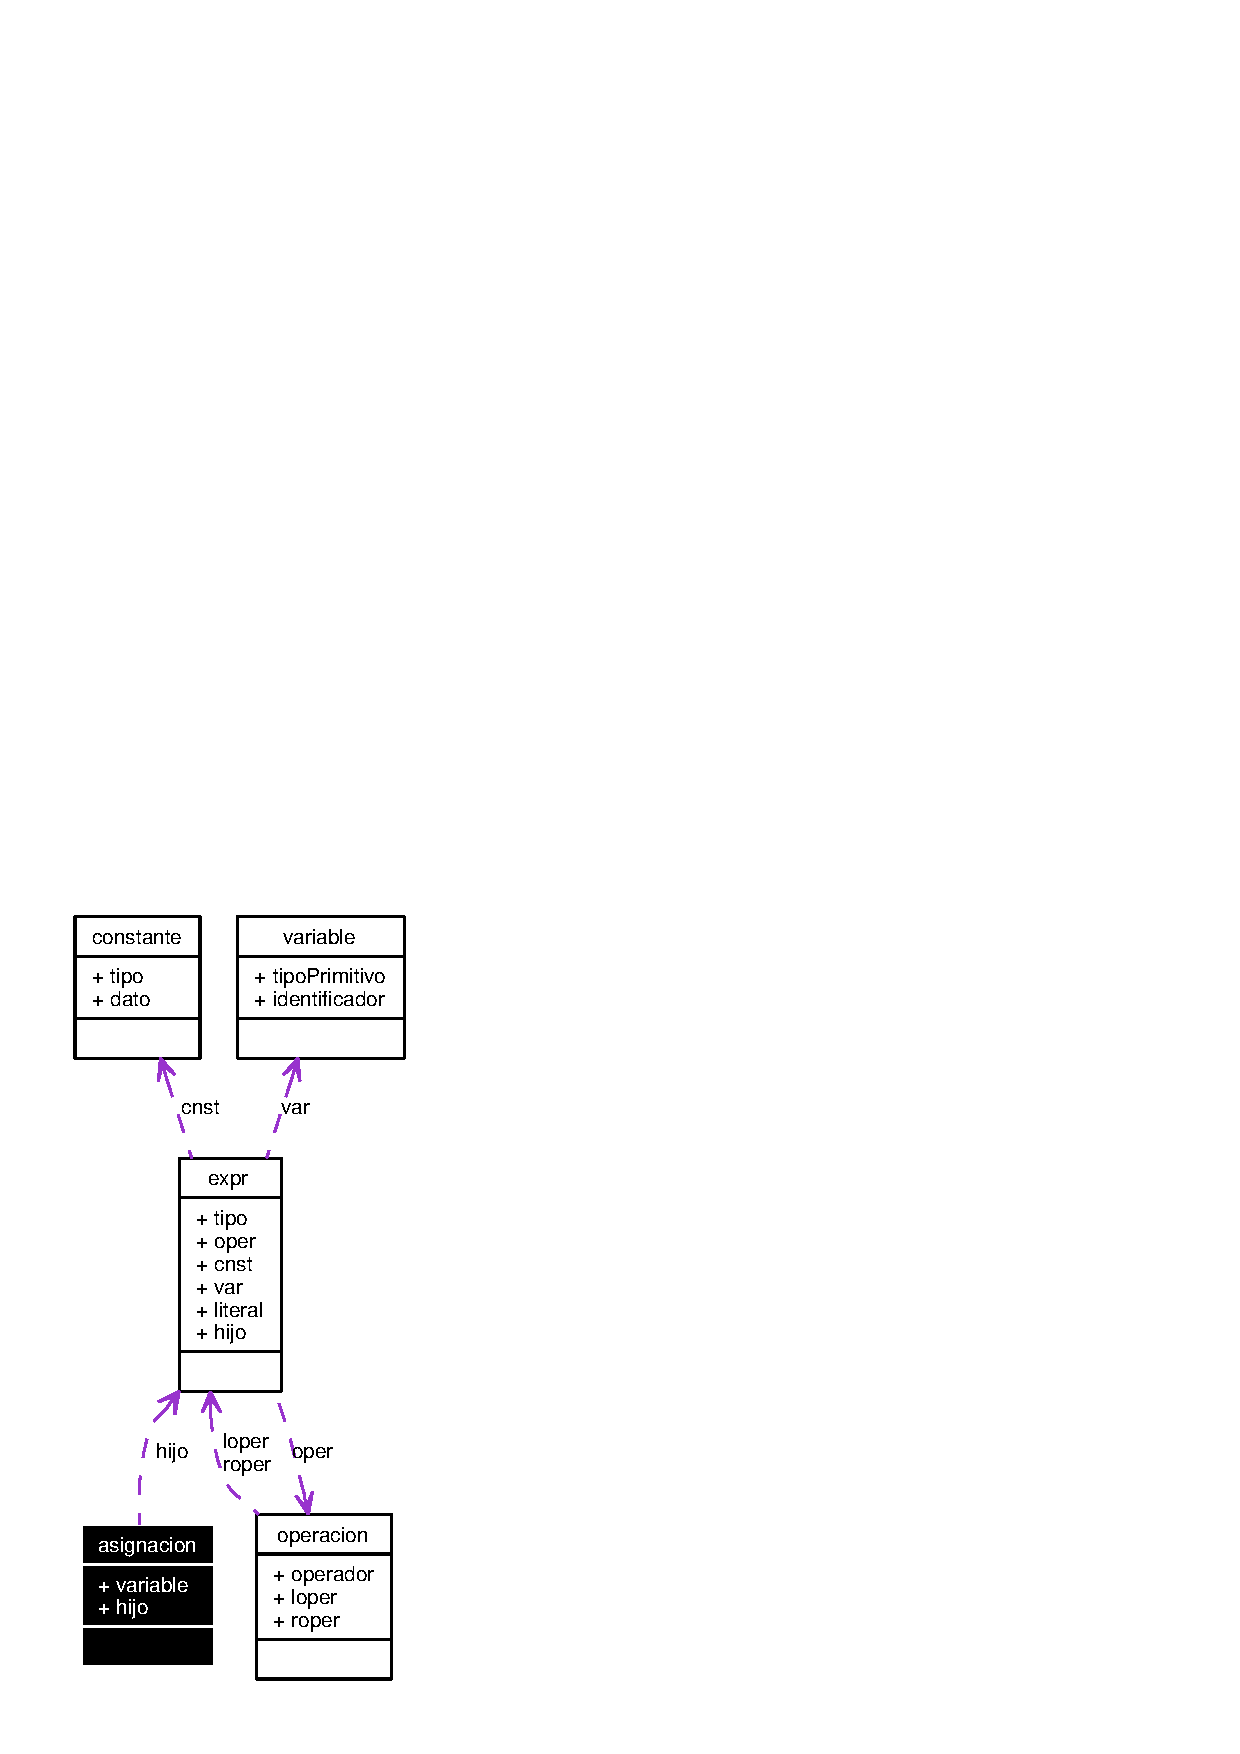
\includegraphics[width=97pt]{structasignacion__coll__graph}
\end{center}
\end{figure}
\subsection*{Atributos p\'{u}blicos}
\begin{CompactItemize}
\item 
char $\ast$ {\bf variable}
\begin{CompactList}\small\item\em Identificador de variable a asignar. \item\end{CompactList}\item 
{\bf expr} $\ast$ {\bf hijo}
\begin{CompactList}\small\item\em Expresion a evaluar para asignar valor. \item\end{CompactList}\end{CompactItemize}


\subsection{Descripci\'{o}n detallada}
Clase de almacenamiento de una asignacion en el AST. 



Definici\'{o}n en la l\'{\i}nea 216 del archivo ast.h.

\subsection{Documentaci\'{o}n de los datos miembro}
\index{asignacion@{asignacion}!hijo@{hijo}}
\index{hijo@{hijo}!asignacion@{asignacion}}
\subsubsection{\setlength{\rightskip}{0pt plus 5cm}{\bf expr}$\ast$ {\bf asignacion::hijo}}\label{structasignacion_o1}


Expresion a evaluar para asignar valor. 



Definici\'{o}n en la l\'{\i}nea 218 del archivo ast.h.

Referenciado por borrar\-Asignacion(), evaluar\-Asignacion(), y insertar\-Asignacion().\index{asignacion@{asignacion}!variable@{variable}}
\index{variable@{variable}!asignacion@{asignacion}}
\subsubsection{\setlength{\rightskip}{0pt plus 5cm}char$\ast$ {\bf asignacion::variable}}\label{structasignacion_o0}


Identificador de variable a asignar. 



Definici\'{o}n en la l\'{\i}nea 217 del archivo ast.h.

Referenciado por borrar\-Asignacion(), evaluar\-Asignacion(), y insertar\-Asignacion().

La documentaci\'{o}n para esta estructura fu\'{e} generada a partir del siguiente archivo:\begin{CompactItemize}
\item 
/media/docs/progra/c++/compiladores1/proy2/godzilla/src/{\bf ast.h}\end{CompactItemize}
